\begin{subfigure}{.9\columnwidth}
	\centering
	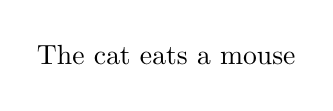
\begin{tikzpicture}[every node/.style={align=center, minimum height=2em, minimum width=1cm}]
		\Tree [ .\node{The cat eats a mouse}; {A} {B} ]
	\end{tikzpicture}
	\caption{Labelled tree representing the equivalent parsing diagram to
		\ref{fig:parsing-diagram}}
\end{subfigure}

\medskip

\begin{subfigure}{.9\columnwidth}
	\centering
	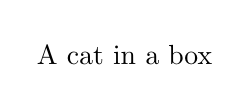
\begin{tikzpicture}[every node/.style={align=center, minimum height=2em, minimum width=1cm}]
		\Tree [ .\node{A cat in a box}; {C} {D} ]
	\end{tikzpicture}
	\caption{Labelled tree representing the equivalent parsing diagram to
		\ref{fig:parsing-diagram2}}
\end{subfigure}

\medskip

\begin{subfigure}{.9\columnwidth}
	\centering
	\begin{tikzpicture}[every node/.style={align=center, inner sep=6pt}, level distance=1.5cm]
		\Tree [
		.\node[comb={$>$}]{\t \\ $\mathbf{if}(\forall x. \w{pass} x)\w{rain}$};
		[ .\node[comb={$>$}]{$\t \to \t$ \\ $\mathbf{if}(\forall x.\w{pass} x)$};
		{$\t \to \t \to \t$ \\ if}
		[
		.\node{$\t$\\ $\forall x. \w{pass} x$ \\ $\combDN_{\Downarrow_{\f{C}}}$};
		[ .\node[comb={$\combMR_{\f{C}}<$}]{$\f{C}\t$ \\ $\lambda c.\forall x. c(\w{pass} x)$};
		{$\f{C}\e$ \\ $\lambda c. \forall x. c\, x$ \\ everyone}
		{$\e \to \t$ \\ $\mathbf{pass}$ \\ passed}
		]
		]
		]
		[
		.{\t \\ $\mathbf{rain}$} \edge[roof]; {it was raining}
		]
		]
	\end{tikzpicture}
	\caption{Labelled tree representing the equivalent parsing diagram to
		\ref{fig:3dparsing-diagram}}
\end{subfigure}
